\section{Results}

\subsection{Training comparison}
\begin{figure}[H]
	\centering
	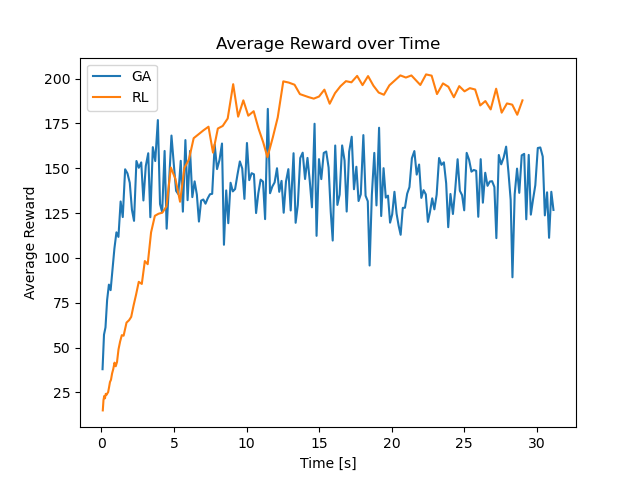
\includegraphics [scale = 0.5]{Images/RL_GA_comparison_avg.png}
	\caption{placeholer}
	\label{figAVG}
\end{figure}

\begin{figure}[H]
	\centering
	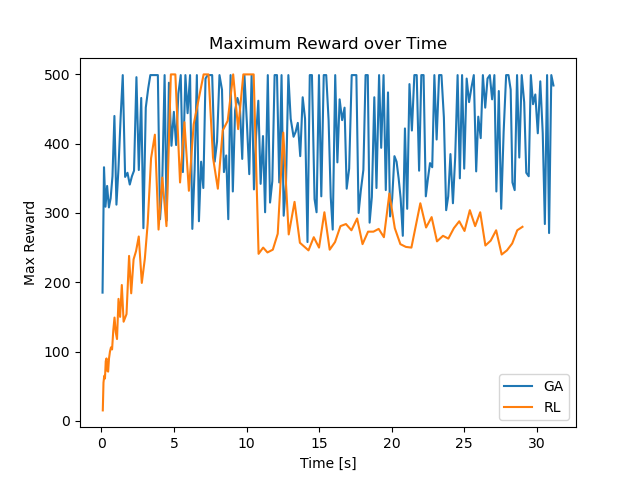
\includegraphics [scale = 0.5]{Images/RL_GA_comparison_max.png}
	\caption{placeholer}
	\label{figMAX}
\end{figure}



\subsection{final model comparison}

\begin{figure}[H]
	\centering
	
\includegraphics [scale = 0.7]{Images/diff.png}
	\caption{Difference between the two state action tables obtained using GA and RL. The black pixels represents the states where choosen action is the same, white pixels represent a different action's choice. The x-axis contains all the possible pairs of the first two elements of the state's 4D-vector, $(s_1,s_2)$, y-axis all the possible pairs of the last two elements $(s_3,s_4)$. }
	\label{figTABLEDIFF}
\end{figure}

% % Delete the text and write your Results here:
% %------------------------------------

% The results section can be combined with the discussion if appropriate. In case of many sub\-/experiments % \-/ fixes the problem that LaTeX won't hyphenate words with dashes in them.
% where the results are vaguely related or unrelated, it would be appropriate to combine the results and discussion. This way you have the information related to each sub-experiment gathered in one place. \par
% Provide uncertainties for the results, but don't discuss it. Do not involve personal opinions, just present the cold hard results in form of numbers, tables, graphs and some sentences. \par
% \Cref{tab:Some-numbers} shows a nice table with comma alignment. \par

% \begin{table}[htb]%
% \centering
% \caption{Table with comma alignment.}
% 	\label{tab:Some-numbers}
% 	\begin{tabular}{SSS} 		% S = special column format from the siunitx package. Aligns commas.
% 		\toprule
% 		{$m$}  &  {$a$}  & {$F$}  \\
% 		{(\si{kg})} &  {(\si{m.s^{-2}})} & {(\si{N})}  \\
% 		\midrule
% 		1,2 & 10,1 & 12 \\
% 		2,44 & 6,92 & 16,88 \\
% 		10 & 1,0 & 10 \\
% 		8,2 & 1,1 & 9,0 \\
% 		100 & 1 & 100 \\
% 		\bottomrule
% 	\end{tabular}
% \end{table}

